\documentclass[10pt,a4paper]{article}
\usepackage{graphicx}
\usepackage[utf8]{inputenc}
\usepackage{amsmath}
\usepackage{amsfonts}
\usepackage{amssymb}
\author{TCP Solutions}
\title{Main project SRS}

\begin{document}

\begin{titlepage}
\begin{center}

\huge Software Requirements Specification\\[0.15cm]
\huge Forensic Medicine Field Guide Template\\[0.15cm]
\large \texttt{Version: 1.0}\\[1cm]

Organization:\\
\texttt{University of Pretoria: TCP Solutions}\\[0.5cm]
GitHub:\\[0.01cm]

\begin{verbatim}
          https://github.com/CollenMphabantshi/TCP-Solutions
\end{verbatim}

Authors:\\
\texttt{Mr Mphambantshi C (10404687)\\
        Mr Legodi PT (29302732)\\
        Ms Sikhitha TP  (10404687)}\\[1cm]
        
May 22, 2014

\begin{tabular}{|l|l|l|}\hline
Name   & Date	& Changes	\\\hline
TP Solutions	& 14 May 2014	& Vision and Scope\\\hline
TP Solutions	& 15 May 2014	& Addition to vision and scope and quality requirements.\\\hline
TP Solutions	& 16 May 2014	& Software Architecture\\\hline
\end{tabular}

\end{center}
\end{titlepage}


\tableofcontents
\pagebreak
\section{Overview}

\subsection{Assumtions}
The purpose of this document is to form a legally binding common ground between clients and the developers. This document will stipulate the functional and non-functional requirements of a system that will allow various contributors to collect, navigate information at the death scene, as well to allow the honors and masters students to view case information that is cleared for them.

\subsection{Overview of documents and when they are created}


\subsection{Document conventions}
\begin{description}
\item Documentation formulation: LaTeX
\item Unified Modelling Language: version 2.0
\end{description}

\section{Vision and Scope}
The proposed system is the death scene register that allow:
 \begin{itemize}
 \item Forensic officers to: 
	 \begin{itemize}
		\item Capture data from death scene.
		\item View basic information.
		\item Reporting.
	\end{itemize}
\item Forensic practitioner to:
	 \begin{itemize}
		\item Generate reports.
		\item View all cases.
		\item Edit case information.
		\item Manage cases.
	 \end{itemize}
\item Students to:
	 \begin{itemize}
		\item View all the cases cleared to them.
	 \end{itemize}
\item Administrator to:
	 \begin{itemize}
		\item Add new users.
		\item Remove users.
		\item Edit users.
		\item View audit report.
	 \end{itemize}
\end{itemize}
\begin{center}
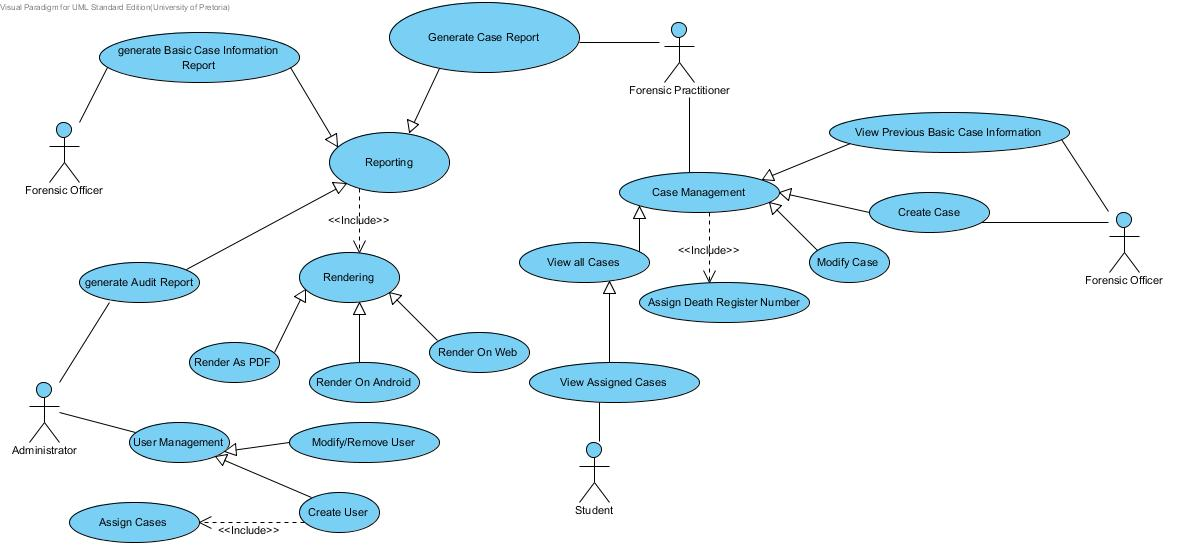
\includegraphics[scale=0.5]{DRUC.jpg}
\end{center}

\pagebreak
\section{Architecture requirements}
\subsection{Access channel requirements}
\indent\indent \textbf{Browser Clients}
\begin{itemize}
\item The browser clients that would be able to access the application from different platforms are as follows...
\begin{itemize}
\item Google Chrome, FireFox Mozilla, Internet Explorer and Safari and any web browsers that run on conventional computers as well as tablets and mobile phones.
\item Because this access channel is architecture independent, it is cross platform.                                                               
\end{itemize}
\end{itemize}
\indent\indent \textbf{Application client}
\begin{itemize}
\item The Android clients that would be able to access the application are as follows...
\begin{itemize}
\item Any Android device that has an Android API level greater or equal to 14 can use the application.
\end{itemize}
\end{itemize}                                
\indent\indent \textbf{RESful}
\begin{itemize}
\item This is the access channel segment that handles network communication with the database and passes requests to it, as well as accept responses from it.
\end{itemize}                                                                
\indent\indent\textbf{Database}
\begin{itemize}
\item The database that is used for data storage, management, manipulation will be instantiated using MySQL.
\end{itemize}                                                                                                
\subsection{Quality requirements}
\indent\indent\textbf{Scalability}
                               \begin{itemize}
                                                \item The system is vastly scalable and should be able to handle a moderately large amount of users, before the performance starts deteriorating.
                                                \begin{itemize}
                                                                \item The application uses a centralized MySQL database, and all the users across the different platforms will connect to it and communicate with it. 
                                                                \item The approximation of the maximum number of users that MySQL can handle before performance seizes to be optimal is about 150,000 users, this is due to the fact that the application uses this centralized MySQL database, and based on the MySQL documents it can handle about that amount, performing roughly a maximum of 4,294,967,295 connections to the database. 
                                                \end{itemize}
                                \end{itemize}
                \begin{itemize}
                        \item The system provides resource management utilities that cater to the performance and reliability of the system. Examples of these are thread, object and connection pooling amongst others.
                        \begin{itemize}
                                \item Making the performance independent to the number of number of users.
                        \end{itemize}
                \end{itemize}
                \begin{itemize}
                        \item The system supports clustering and load balancing.
                \end{itemize}
                \begin{itemize}
                        \item Connection to the Database is persistent, and connection can only be lost when the users decide to terminate the connection.\\
                \end{itemize}

\indent\textbf{Authentication}
                \begin{itemize}
                        \item The users have to have an account in order access the application; this will provide the users with a username and password. These associated pieces of information are important as they will be required for the authentication process i.e. logging.
                        \begin{itemize}
                                \item A user will have to provide his or her username as well as their associated password in order for them to be logged in and for a session to be created for them.
                        \end{itemize}
                \end{itemize}
                \begin{itemize}
                        \item The Session that is created when the user logs in with continues be checked for authentication throughout the time that the user is accessing the application. These checks could be done when the state of the application changes, when a request is sent or after a specified period of time.
                        \begin{itemize}
                                \item If the authentication fails at any point, then the user will be kicked out of the system and will be forced to try to log in again.
                        \end{itemize}
                \end{itemize}

\indent\textbf{Authorization}
                \begin{itemize}
                        \item Authorization tokens will be assigned to each user, irrespective of the sort of account that they may hold.
                        \begin{itemize}
                                \item The tokens determine the users privileges.
                        \end{itemize}
                        \begin{itemize}
                                \item They also determine what the user is allowed to read  e.g view all the marks or just specific ones.
                        \end{itemize}
                        \begin{itemize}
                                \item They determine whether a user can modify marks or any specific fields at all.
                        \end{itemize}
                        \begin{itemize}
                                \item They determine whether a user can execute certain actions on the application.
                        \end{itemize}
                \end{itemize}
                \begin{itemize}
                        \item
                        The privileges layers that the tokens offer can be elevated /promoted to a lower state or a higher state with 0 being the most privileged state as depicted in diagram.\linebreak\linebreak \begin{center}
                        
                        
                        \begin{tabular}{|c|c|}\hline
                        Tokens   & Privileges \\\hline
                        n & More privileges then level n+1\\\hline
                        1 & Less privileges then level 0\\\hline
                        0 & Most privileged\\\hline
                \end{tabular}
                \end{center}
                \end{itemize}
\pagebreak
\indent\indent\textbf{Security}
                \begin{itemize}
                        \item The passwords that are assigned are assigned to each user are encrypted using a sophisticated encryption algorithm called the “message-digest algorithm” otherwise known as md5.
                        \begin{itemize}
                                \item  This algorithm prevents people who have access to the control (database) from being able to view the actual password and associate it with the user name and thus seize control of a user’s account.
                        \end{itemize}
                        \end{itemize}

                \begin{itemize}
                        \item  When a user’s fails to provide the correct login parameters 3 times in a row, the user account is suspended for 10 minutes.
                        \begin{itemize}
                                \item  The idea is to try and prevent bots (computer programs that try all the possible password combinations) from accessing an account,  any users account.
                        \end{itemize}
                \end{itemize}

\indent\textbf{Audit-ability}
                \begin{itemize}
                        \item  Once the users have successfully logged into the application, they have the ability to perform certain tasks depending on their assigned privilege tokens.
                        \end{itemize}
                \begin{itemize}
                        \item The users activity is logged in detail so that they can be referred to later if need be. Some of the activates that are logged are as follows…

                        \begin{itemize}
                                \item Changes to fields or rows in the database.
                        \end{itemize}
                        \begin{itemize}
                                \item Updates to fields or rows in the database.
                        \end{itemize}
                        \begin{itemize}
                                \item Additions to any aspect of the database.
                        \end{itemize}
                        \begin{itemize}
                                \item The execution of activities that directly or indirectly affect the database or another user.
                        \end{itemize}
                \end{itemize}						
                         
\indent\textbf{Reliability}         
          
	\begin{itemize}
		\item There will be easy and fast access to the database.
		\item The system will save made changes if the system crashed while the user was working
		\item Users can still resume their sessions, if the device closed the application for some reason (e.g battery died).
		\item Errors will be handled and the system will show enough information about the errors.
		\item In a situation when a database crashed. There will be a backup database used to recover within a reasonable time.
	\end{itemize}
	\pagebreak
\indent\indent\textbf{Availability}       
        \begin{itemize}
                \item Online vs offline db connect
                \item Local database must be utilized when mobile interface is offline.
                \item Local database must synchronise with server once it is online.
                
		\item The system will be available in different platforms. Users can either access the system using mobile devices or by using any device with a web browser.
		\item The system can also be accessed anytime and anywhere.
		\item Inputs will be validated to prevent errors, before the execution of any input command.
		\item If the server is down the services or requests can be redirected to the backup server.
	 
        \end{itemize}   
                                                      
\indent\textbf{Flexibility}         
        \begin{itemize}
                \item The system will use SOAP based services, where changes to some of the parts of the service will not affect the design and some functionality of the system.
		\item The system allows integration with other systems.
		\item The system will take into account if the user loses internet connection or for whatever reason they cannot establish a connection to the server. The user can still be able to use the application but any transaction done while the system is disconnected will be cached until the connection is restored.
		\item Object Oriented Programming will be used to allow changes to some parts of the code(program). Those changes will not affect other objects. Reason for this would be to allow the system's design and implementations to be reusable for upgrading the system later on for new platforms.
        \end{itemize}   

\indent\textbf{Performance}         
        \begin{itemize}
                \item System should respond in timely fashion allowing markers to work at the quickest pace possible.
        \end{itemize}  
 
\subsection{Integration requirements}
	\indent\indent\textbf{LDAP}
    \begin{itemize}
                \item The system is used for the authentication requirements of the application.\\This ranges from user login authentication to the permission based token assignment.
    \end{itemize}
    
	\textbf{SOAP}
    \begin{itemize}
                \item This protocol does the communication within the network. It achieves this by accepting request and sending responses to and from different interfaces and processing them accordingly.\\e.g.Receiving a request to view marks from an android application interface and passing the request to the database, then returning the result.  
    \end{itemize}   
    
	\textbf{ADOBE API}
    \begin{itemize}
                \item This API is used when generating a report. The result is then presented as a PDF using the fore mentioned API. 
    \end{itemize}   


	\textbf{Mark API}
	\begin{itemize}
		\item Must interface with CS website login details.
		\item Must use Soap interface through out all applications.
		\item Must Facilitate marking sessions.
		\item Marking sessions must coincide with practical sessions.
		\item Marking session durations must also be personalizable by the client.
		\item Marker(s) must be able to record marks during marking sessions.
		\item Marks must be stored in a database.
		\item Database must be exportable to a .csv file.
		\item Database must have lock/unlock capabilities that are also automated depending on whether are marking session is currently happening.
		\item Unlocked databases must allow marker(s) to alter marks.
		\item Altered marks must include reason for alteration.
		\item Marker(s) must be able to alter marks from previous marking session only with the permission/knowledge of the client.
	\end{itemize}
		
	\textbf{Booking API} \newline
	\indent Must interface with Computer Science website booking system. 
                
\subsection{Architecture constraint}
       \begin{itemize}
                \item Architecture: Waterfall Architecture 
        \end{itemize}
       \begin{itemize}
                \item Database technology: MySQL
        \end{itemize}
                \begin{itemize}
                        \item  It must run using HTTPS requests and response events to connect to the database.
                \end{itemize}
                \begin{itemize}
                        \item Authentication: LDAP (LOGIN)                 
                                \end{itemize} 
                \begin{itemize}
                        \item Importable Data Format: CSV
                \end{itemize}
                \begin{itemize}
                        \item Exportable Data Format: CSV
                \end{itemize}
                \begin{itemize}
                        \item Interface: SOAP
                \end{itemize}
                \begin{itemize}
                        \item Server communication: Django
                \end{itemize}
                \begin{itemize}
                        \item Security/Authentication: LDAP
                \end{itemize}
                \begin{itemize}
                        \item Text encoding: UTF-8
                \end{itemize}
                \begin{itemize}
                        \item Client interface platforms
                                                        \begin{itemize}
                                                                \item Android
                                                                \item Web browser
                                                                \item Cross Compatible OS support for Linux, Mac OS X and Windows
                                                                \item Any sensitive information stored must be stored in encrypted format.
                                                        \end{itemize}                                           
                \end{itemize}                                           
                
\section{Functional Requirements}
\subsection{Introduction}
This project ,when finalized, should act as a holistic marks management system. The system will have different privilege levels, when assigned to a level , users will have a restricted set of tools stipulated as follows: 
\begin{enumerate}
\item Level 0. This level can be seen as a level with "root" privileges. It is intended to only be assigned to either one or two people and will give access to all level 1, 2 ,3 and 4 privileges as well as be able to add and remove subjects from the system. 
\item Level 1 users (such as Students) should be able to view their own marks.
\item Level 2 users (such as Teaching Assistants and Tutors) will be able to view any students marks that are in a session that the level 2 person is assigned to. This level will also give access to adding as well as modifying marks.
\item Level 3 users (such as lecturers) will be able to configure mark roll-ups, add assessment opportunities and draw reports from all of the marks of the subjects of which he is assigned to. This level will also have all of the privileges of level 1 as well as level 2 users.
\end{enumerate}
These tools will be available in a web based interface as well as an Android interface.


\subsection{Scope and Limitations}

\begin{center}
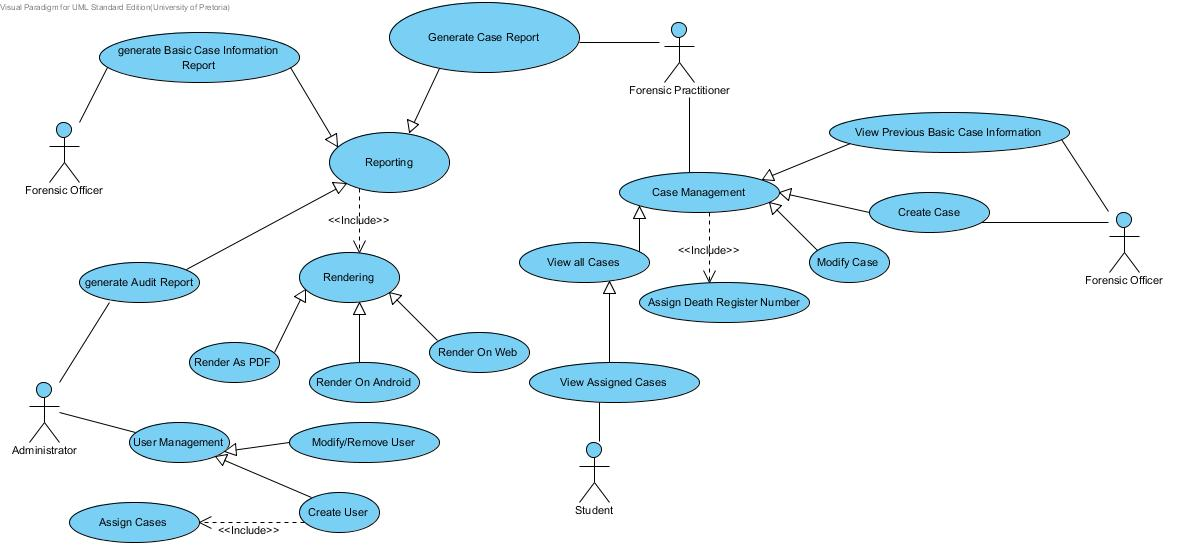
\includegraphics[scale=0.5]{DRUC.jpg}
\end{center}


\subsection{Required functionality}




\subsection{Use case prioritization}

\textbf{Critical:}
 \begin{itemize}
	\item Security, the system must be secure to protect the marks.

	\item login, must be able to differenciate between users. 

	\item Auditing, must record changes made to the system for safety. 

	\item Booking, must get the information from the cs website.

	\item Assessments, must state the different practicals, test ens.

	\item Marks, the system is made to collect marks.
 \end{itemize}
 
 
 
\textbf{Important:}
\begin{itemize}
	\item Course, the system is used by multiple courses.

	\item Course configuration, add and remove user.
 \end{itemize}

\textbf{Nice-To-Have:}
 \begin{itemize}
	\item Reporting, different ways the view the information and allowing students do draw simple reports.

	\item View course, view extra information.

	\item Flagging, adding flags to irregularities.
 \end{itemize}


\subsection{Use case/Services contracts}
 \begin{tabular}{|l|l|}\hline
                        Use Case Name   & Login \\\hline
                        Reference & Section 1.1\\\hline
                        Trigger & The user accesses the login page of the application.\\\hline
                        Precondition & The user must enter the correct username and password.\\\hline
                        Basic Path & 1.	The user enters his/her login details and submits. 
                        \\\linebreak &
                        2.	 The system verifies that the information provided is valid.
                        \\\hline
                        Alternative & In step 2 if the information provided is invalid, the system will
                        \\\linebreak & return the user to the login page.\\\hline
                        Postcondition & The home page will be displayed.\\\hline
                \end{tabular} 
                
                \begin{tabular}{|l|l|}\hline
                        Use Case Name   & Auditing \\\hline
                        Reference & Section 1.2\\\hline
                        Trigger & The user changes in formation on the system.\\\hline
                        Precondition & The user must be logged in.\\\hline
                        Basic Path & 1.	The user performs an action that changes information on the
                        syetem. \\\linebreak & 
                        2.	 The system logs the change and the user, with date and time.\\\hline
                        Alternative & N/A\\\hline
                        Postcondition & The information will be logged in the audit log.\\\hline
                \end{tabular} \\\linebreak           
                
                \begin{tabular}{|l|l|}\hline
                        Use Case Name   & Booking \\\hline
                        Reference & Section 2.1\\\hline
                        Trigger & The user logs in.\\\hline
                        Precondition & The system must be connected to the cs website.\\\hline
                        Basic Path & The user enters the home page.\\\hline
                        Alternative & The system can't access the cs website and  
                        \\\linebreak & an error message is displayed.\\\hline
                        Postcondition & The system displays the booking information.\\\hline
                \end{tabular} \\\linebreak
                
  
                \begin{tabular}{|l|l|}\hline
                        Use Case Name   & Assessments \\\hline
                        Reference & Section 2.2\\\hline
                        Trigger & The user accesses an assessment.\\\hline
                        Precondition & The assessment must be available.\\\hline
                        Basic Path & 1.	The user selects an assessment like a practical, test ens.\\\hline
                        Alternative & There is no assessment to be selected.\\\hline
                        Postcondition & The assessment information will be displayed.\\\hline
                \end{tabular}\\\linebreak
                
                \begin{tabular}{|l|l|}\hline
                        Use Case Name   & Marks \\\hline
                        Reference & Section 2.2.5\\\hline
                        Trigger & The user selects the marks of an assessment.\\\hline
                        Precondition & The user must have selected an assessment.\\\hline
                        Basic Path & 1.	The user marks to display the options available for marks.\\\hline
                        Alternative & There is no marks available\\\hline
                        Postcondition & The options is given to CRUD the marks.\\\hline
                \end{tabular}\\\linebreak
                
                \begin{tabular}{|l|l|}\hline
                        Use Case Name   & View course \\\hline
                        Reference & Section 2.3\\\hline
                        Trigger & The user selects view course.\\\hline
                        Precondition & The course must be available.\\\hline
                        Basic Path & 1.	The user selects the course he wants to view.\\\hline
                        Alternative & No courses are available.\\\hline
                        Postcondition & The course information will be shown.\\\hline
                \end{tabular}\\\linebreak
                
                \begin{tabular}{|l|l|}\hline
                        Use Case Name   & Course configuration \\\hline
                        Reference & Section 1.1\\\hline
                        Trigger & The user selects course configuration.\\\hline
                        Precondition & The user must have the right security priviliges.\\\hline
                        Basic Path & 1.	The user selects course configurations. \\\linebreak &
                        2.	 The changes the configurations.\\\hline
                        Alternative & The user does not have the right security priviliges.\\\hline
                        Postcondition & The configurations for the course is changed.\\\hline
                \end{tabular}\\\linebreak
                
                
                
               
\pagebreak

\section{Open Issues}
The Minimum Android API level to be supported by the Android application was not properly specified by the client. The selected API level was selected trying to accommodate as many devices as possible. A potential issue can occur if the students are using a Android device that is too old. An issue which should be resolved by having the web interface.
\section{Glossary}
\begin{description}
	\item[API] Application Program Interface specifying how some software components should interact with each other.
	\item[db] Database
	\item[HTTPS] Hypertext Transfer Protocol Secure is a communications protocol for secure communication over a computer network, with especially wide deployment on the Internet.
	\item[md5] The MD5 message-digest algorithm is a widely used cryptographic hash function that produces a 128-bit hash value.
	\item[MySQL] MySQL (Structured Query Language) is an open-source relational database management system.
	\item[OS] Operating System
	\item[PDF] Portable Document Format is a file format for capturing and sending electronic documents in exactly the intended format.
	\item[UML] Unified Modelling Language is a general-purpose modelling language in the field of software engineering. It provides a set of graphic notation techniques to create visual models of object-oriented software-intensive systems. 
	\item[UTF-8] A variation of UTF (Unicode Transformation Format) which is a variable-width encoding that can represent every character in the Unicode character set.
	\pagebreak
	\begin{center}

	\end{center}
	\item[Level[M:N]] Means from security level M up until security level N.
		
\end{description}

\end{document}
